% !TEX program = xelatex
% =====================================================================
%  JSTT (Journal of Science and Transport Technology) - UTT
%  Single-file template for Overleaf
%  Compile with XELATEX
% =====================================================================
\documentclass[10pt]{article}

%---------------------------------------------------------------------
% Font (XeLaTeX)
%---------------------------------------------------------------------
\usepackage{fontspec}
\IfFontExistsTF{Arial}{%
  \setmainfont{Arial}
}{%
  \IfFontExistsTF{Liberation Sans}{%
    \setmainfont{Liberation Sans}
  }{%
    \setmainfont{TeX Gyre Heros}
  }%
}

%---------------------------------------------------------------------
% Geometry - A4 portrait
%---------------------------------------------------------------------
\usepackage[a4paper,top=2.6cm,bottom=2.2cm,left=1.8cm,right=1.8cm,columnsep=6mm]{geometry}

%---------------------------------------------------------------------
% Packages
%---------------------------------------------------------------------
\usepackage{graphicx}
\usepackage{amsmath,amssymb}
\usepackage{array}
\usepackage{tabularx}
\usepackage{booktabs}
\usepackage{colortbl}
\usepackage{fancyhdr}
\usepackage{titlesec}
\usepackage{enumitem}
\usepackage{xcolor}
\usepackage{caption}
\usepackage{subcaption}
\usepackage{multicol}
\usepackage{ragged2e}
\usepackage{float}
\usepackage{setspace}
\usepackage{calc}
\usepackage{tikz}

%---------------------------------------------------------------------
% Colors
%---------------------------------------------------------------------
\definecolor{jsttbg}{HTML}{DDD9C3}
\definecolor{jsttblue}{HTML}{003366}
\definecolor{jsttcite}{HTML}{0055A5} % Màu xanh chuẩn link & text tài liệu tham khảo

% Cấu hình Hyperref: Màu xanh link trích dẫn và liên kết web
\usepackage[colorlinks=true,linkcolor=black,citecolor=jsttcite,urlcolor=jsttcite]{hyperref}

% Đổi màu số thứ tự [1], [2]... trong danh mục Tài liệu tham khảo thành màu xanh
\makeatletter
\renewcommand{\@biblabel}[1]{\textcolor{jsttcite}{[#1]}}
\makeatother

%---------------------------------------------------------------------
% Figure/Table names
%---------------------------------------------------------------------
\renewcommand{\figurename}{Hình}
\renewcommand{\tablename}{Bảng}
\renewcommand{\refname}{Tài liệu tham khảo}

%---------------------------------------------------------------------
% Line spacing & paragraph
%---------------------------------------------------------------------
\linespread{1.2}
\setlength{\parindent}{0pt}
\setlength{\parskip}{6pt}

%---------------------------------------------------------------------
% Section formatting
%---------------------------------------------------------------------
\renewcommand{\thesection}{\arabic{section}}
\renewcommand{\thesubsection}{\thesection.\arabic{subsection}}
\renewcommand{\thesubsubsection}{\thesubsection.\arabic{subsubsection}}

\titleformat{\section}
  {\bfseries\fontsize{11}{13}\selectfont}{\thesection.}{0.4em}{}
\titleformat{\subsection}
  {\bfseries\fontsize{10}{12}\selectfont}{\thesubsection.}{0.4em}{}
\titleformat{\subsubsection}
  {\bfseries\fontsize{9}{11}\selectfont}{\thesubsubsection.}{0.4em}{}
\titlespacing*{\section}{0pt}{8pt}{4pt}
\titlespacing*{\subsection}{0pt}{6pt}{3pt}
\titlespacing*{\subsubsection}{0pt}{4pt}{2pt}

%---------------------------------------------------------------------
% Caption formatting
%---------------------------------------------------------------------
\captionsetup[figure]{labelfont=bf,font={footnotesize},justification=centering,skip=4pt}
\captionsetup[table]{labelfont=bf,font={footnotesize},justification=raggedright,singlelinecheck=false,skip=4pt}

%---------------------------------------------------------------------
% Header & Footer (from page 2 onward)
%---------------------------------------------------------------------
\pagestyle{fancy}
\fancyhf{}
\renewcommand{\headrulewidth}{0.6pt}
\renewcommand{\footrulewidth}{0pt}
\fancyhead[L]{\fontsize{7}{8}\selectfont\itshape JSTT vol 6(2026), 4, 11-25}
\fancyhead[R]{\fontsize{7}{8}\selectfont\itshape V. D. Vinh et al.}
\fancyfoot[L]{\fontsize{7}{8}\selectfont JSTT 2026, 6, 4, 11-25. \href{https://doi.org/10.58845/jstt.utt.2026.vn.6.4.11-25}{doi.org/10.58845/jstt.utt.2026.vn.6.4.11-25}}
\fancyfoot[R]{\fontsize{7}{8}\selectfont \href{https://jstt.vn/index.php/vn}{jstt.vn}}
\fancyfoot[C]{\fontsize{9}{10}\selectfont\thepage}

\fancypagestyle{firstpage}{%
  \fancyhf{}
  \renewcommand{\headrulewidth}{0pt}
  \fancyfoot[L]{\fontsize{7}{8}\selectfont JSTT 2026, 6, 4, 11-25. \href{https://doi.org/10.58845/jstt.utt.2026.vn.6.4.11-25}{doi.org/10.58845/jstt.utt.2026.vn.6.4.11-25}}
  \fancyfoot[R]{\fontsize{7}{8}\selectfont \href{https://jstt.vn/index.php/vn}{jstt.vn}}
  \fancyfoot[C]{\fontsize{9}{10}\selectfont\thepage}
}

%---------------------------------------------------------------------
% Graphics path
%---------------------------------------------------------------------
\graphicspath{{./}{./images/}}

%---------------------------------------------------------------------
% Safe includegraphics
%---------------------------------------------------------------------
\newcommand{\safeincludegraphics}[2][]{%
  \IfFileExists{#2}{%
    \includegraphics[#1]{#2}%
  }{%
    \fbox{\parbox[c][1.2cm][c]{2.5cm}{\centering\scriptsize Image}}%
  }%
}

%---------------------------------------------------------------------
% JSTT Header - Tiếng Việt
%---------------------------------------------------------------------
\newcommand{\JSTTHeader}{%
\noindent
% Đường kẻ ngang trên cùng
\rule{\textwidth}{1.3pt}\par
\vspace{5pt}

\noindent
\begin{minipage}[c]{0.17\textwidth}
  % Logo JSTT bên trái
  \includegraphics[width=\linewidth, height=1.95cm, keepaspectratio]{images/Picture1.png}
\end{minipage}%
\hfill
\begin{minipage}[c]{0.63\textwidth}
  % Banner giữa
  \colorbox{jsttbg}{%
    \begin{minipage}[c][1.95cm][t]{\dimexpr\linewidth-2\fboxsep\relax}
      \fontspec{Times New Roman}
      \vspace{0.14cm}
      {\centering
        {\fontsize{15}{18}\selectfont Tạp chí điện tử}\\[3pt]
        {\fontsize{15}{18}\selectfont Khoa học và Công nghệ Giao thông}\par
      }
      % Đẩy toàn bộ khoảng cách thừa lên giữa
      \vfill
      % Dạt phải và giữ lại 2.5pt an toàn để toàn bộ dấu câu nằm trong dải màu
      \raggedleft
      {\fontsize{12.5}{14}\selectfont Đại học Công nghệ Giao thông vận tải}\hspace{0.25cm}\par
      \vspace{2.5pt}% Giữ khoảng thở vừa vặn cho các dấu nặng/móc phía dưới
    \end{minipage}%
  }
\end{minipage}%
\hfill
\begin{minipage}[c]{0.17\textwidth}
  % Logo UTT bên phải
  \raggedleft
  \includegraphics[width=\linewidth, height=1.95cm, keepaspectratio]{images/Picture2.png}
\end{minipage}

\vspace{5pt}
% Đường kẻ đơn phía dưới
\noindent\rule{\textwidth}{1.3pt}\par
}

%---------------------------------------------------------------------
% JSTT Header - English Version
%---------------------------------------------------------------------
\newcommand{\JSTTHeaderEN}{%
\noindent
% Đường kẻ ngang trên cùng
\rule{\textwidth}{1.3pt}\par
\vspace{5pt}

\noindent
\begin{minipage}[c]{0.17\textwidth}
  % Logo JSTT bên trái
  \includegraphics[width=\linewidth, height=1.95cm, keepaspectratio]{images/Picture1.png}
\end{minipage}%
\hfill
\begin{minipage}[c]{0.63\textwidth}
  % Banner giữa
  \colorbox{jsttbg}{%
    \begin{minipage}[c][1.95cm][t]{\dimexpr\linewidth-2\fboxsep\relax}
      \fontspec{Times New Roman}
      \vspace{0.45cm}
      {\centering
        {\fontsize{15}{18}\selectfont Journal of Science and Transport Technology}\par
      }
      % Đẩy toàn bộ khoảng cách thừa lên giữa
      \vfill
      % Dạt phải và giữ lại 2.5pt an toàn cho chân chữ
      \raggedleft
      {\fontsize{13}{15}\selectfont University of Transport Technology}\hspace{0.25cm}\par
      \vspace{2.5pt}
    \end{minipage}%
  }
\end{minipage}%
\hfill
\begin{minipage}[c]{0.17\textwidth}
  % Logo UTT bên phải
  \raggedleft
  \includegraphics[width=\linewidth, height=1.95cm, keepaspectratio]{images/Picture2.png}
\end{minipage}

\vspace{5pt}
% Đường kẻ đơn phía dưới
\noindent\rule{\textwidth}{1.3pt}\par
}

%---------------------------------------------------------------------
% Titlebox - article info (left) + title/abstract (right)
% #1 = article info (left column)
% #2 = title + authors + abstract + keywords (right column)
%---------------------------------------------------------------------
\newcommand{\titlebox}[2]{%
\vspace{\baselineskip} % Cách ra 1 dòng ở đầu trên bảng abstract
\noindent
\setlength{\fboxrule}{0.4pt}
\begin{tabular}{|p{0.28\textwidth}|p{0.69\textwidth}|}
\hline
\begin{minipage}{\dimexpr 0.28\textwidth-2\tabcolsep\relax}
  \vspace{4pt}
  #1
  \vspace{4pt}
\end{minipage} &
\begin{minipage}{\dimexpr 0.69\textwidth-2\tabcolsep\relax}
  \vspace{4pt}
  #2
  \vspace{4pt}
\end{minipage} \\
\hline
\end{tabular}\par
\vspace{\baselineskip} % Cách ra 1 dòng ở đầu dưới bảng abstract
}

%=======================================================================
% DOCUMENT CONTENT
%=======================================================================
\begin{document}
\thispagestyle{firstpage}

% ======================================================================
% TRANG 1: HEADER VÀ ABSTRACT TIẾNG ANH
% ======================================================================
\JSTTHeaderEN

% ========== ENGLISH ==========
\titlebox{%
  \fontsize{8.5}{11}\selectfont
  {\large\bfseries Article info}\\[6pt]
  \textbf{Type of article:}\\[2pt]
  Original research paper\\[6pt]
  \textbf{Corresponding author:}\\[2pt]
  E-mail address:\\[2pt]
  vinh74dctt22119@st.utt.edu.vn\\[6pt]
  \textbf{Received:}\\[3pt]
  \textbf{Accepted:}\\[3pt]
  \textbf{Published:}
}{%
  {\fontsize{11}{13}\selectfont\bfseries\color{jsttblue} An AI-Powered Driver Monitoring System
  Integrating Six Computer Vision Modules for Real-Time Behavior Detection}\\[5pt]
  {\fontsize{9}{11}\selectfont Dao Van Vinh$^{1}$, Nguyen Thanh Xuan$^{1}$, Dao Phuc Dan$^{1}$}\\[3pt]
  {\fontsize{8}{10}\selectfont\itshape
  $^{1}$Faculty of Information Technology, University of Transport Technology, Hanoi, Vietnam}\\[8pt]
  \fontsize{10}{12}\selectfont
  \textbf{Abstract:} \sloppy Drowsiness, inattention, and driving rule violations are leading causes
  of traffic casualties worldwide. Existing driver monitoring solutions are either intrusive
  (physiological sensors) or limited to individual tasks, and no low-cost system integrates
  comprehensive behavioral detection across multiple vision modules. This paper proposes an AI-based
  intelligent driver monitoring system that integrates six computer vision modules: drowsiness,
  yawning, mobile phone usage, seatbelt status, head posture, and steering wheel grip. The system
  employs YOLOv8, MediaPipe, Dlib, and the Perspective-n-Point (PnP) method on a traditional
  three-tier architecture (presentation layer, application layer, data layer). The Flask-based
  application layer integrates a specialized AI inference module for real-time video processing. Experimental results demonstrate
  89,9\% average module accuracy in CPU lab tests and $\sim$92\% end-to-end accuracy with 20--30 FPS on GPU, and 100--200~ms latency, offering a cost-effective real-time
  monitoring solution for enhanced driving safety.\par
  \vspace{\baselineskip} % Cách ra đúng 1 dòng
  \textbf{Keywords:} Driver monitoring; YOLOv8; MediaPipe; Dlib; computer vision;
  traffic safety; edge AI
}

\clearpage

% ======================================================================
% TRANG 2 TRỞ ĐI: HEADER VÀ ABSTRACT TIẾNG VIỆT + NỘI DUNG CHÍNH
% ======================================================================
\JSTTHeader

% ========== TIẾNG VIỆT ==========
\titlebox{%
  \fontsize{8.5}{11}\selectfont
  {\large\bfseries Thông tin bài viết}\\[6pt]
  \textbf{Dạng bài viết:}\\[2pt]
  Bài báo nghiên cứu\\[6pt]
  \textbf{Tác giả liên hệ:}\\[2pt]
  Địa chỉ E-mail:\\[2pt]
  vinh74dctt22119@st.utt.edu.vn\\[6pt]
  \textbf{Ngày nộp bài:} 00/00/2026\\[3pt]
  \textbf{Ngày chấp nhận:} 00/00/2026\\[3pt]
  \textbf{Ngày đăng bài:} 00/00/2026
}{%
  {\fontsize{11}{13}\selectfont\bfseries\color{jsttblue} Hệ thống giám sát tài xế thông minh tích hợp
  sáu module thị giác máy tính phát hiện hành vi thời gian thực}\\[5pt]
  {\fontsize{9}{11}\selectfont Đào Văn Vinh$^{1}$, Nguyễn Thanh Xuan$^{1}$, Đào Phúc Dân$^{1,\ast}$}\\[3pt]
  {\fontsize{8}{10}\selectfont\itshape
  $^{1}$Khoa Công nghệ Thông tin, Trường Đại học Công nghệ Giao thông vận tải, Hà Nội, Việt Nam}\\[8pt]
  \fontsize{10}{12}\selectfont
  \textbf{Tóm tắt:} \sloppy Buồn ngủ, mất tập trung và vi phạm quy tắc lái xe là những nguyên nhân
  hàng đầu gây thương vong giao thông tại Việt Nam. Bài báo đề xuất một hệ thống giám sát tài xế
  thông minh dựa trên trí tuệ nhân tạo, tích hợp 6 module thị giác máy tính bao gồm: phát hiện
  buồn ngủ, ngáp, sử dụng điện thoại, không thắt dây an toàn, tư thế đầu và vị trí tay lái. Hệ
  thống sử dụng các mô hình YOLOv8, MediaPipe, Dlib và phương pháp Perspective-n-Point (PnP) để
  phân tích hành vi tài xế theo thời gian thực. Hệ thống được tổ chức theo kiến trúc ba tầng
  truyền thống gồm tầng giao diện, tầng ứng dụng và tầng dữ liệu, trong đó tầng ứng dụng
  (Flask) tích hợp một module AI suy luận chuyên biệt để xử lý video thời gian thực. Kết quả thực nghiệm
  cho thấy hệ thống đạt 89,9\% trung bình các module trong kiểm thử lab trên CPU và khoảng 92\% end-to-end trên GPU, tốc độ xử lý 20--30 FPS và độ trễ
  đầu cuối 100--200~ms, đáp ứng yêu cầu giám sát thời gian thực và hỗ trợ nâng cao an toàn lái xe.\par
  \vspace{\baselineskip} % Cách ra đúng 1 dòng
  \textbf{Từ khóa:} Giám sát tài xế; YOLOv8; MediaPipe; Dlib; thị giác máy tính;
  an toàn giao thông; AI biên
}

\begin{multicols}{2}

%=======================================================================
% MAIN CONTENT - TWO COLUMNS
%=======================================================================

\section{Giới thiệu}

Tai nạn giao thông đường bộ vẫn là một trong những nguyên nhân hàng đầu gây tử vong và thiệt hại kinh tế trên toàn thế giới. Theo Tổ chức Y tế Thế giới (WHO), mỗi năm có khoảng 1,19 triệu người tử vong và hàng chục triệu người bị thương do tai nạn giao thông đường bộ, trong đó lỗi của người điều khiển phương tiện vẫn là nguyên nhân chủ yếu. Tại Việt Nam, theo báo cáo của Ủy ban An toàn giao thông Quốc gia, giai đoạn 2024--2025 cả nước ghi nhận hơn 6.000 trường hợp tử vong mỗi năm, trong đó tình trạng buồn ngủ, mất tập trung và sử dụng điện thoại khi lái xe là các yếu tố nguy cơ quan trọng dẫn đến nhiều vụ tai nạn nghiêm trọng \cite{hien2026, baogiaothong2025}.

Bên cạnh đó, nhiều nghiên cứu đã chứng minh rằng trạng thái sinh lý và hành vi của người lái ảnh hưởng trực tiếp đến khả năng điều khiển phương tiện. Hiệp hội An toàn giao thông Hoa Kỳ (AAA Foundation for Traffic Safety) cho thấy người lái ngủ dưới 5 giờ trong vòng 24 giờ có nguy cơ gây tai nạn cao gấp 4,5 lần so với người ngủ đủ 7 giờ trở lên \cite{aaa2018}. Tương tự, Cục Quản lý An toàn Giao thông Đường cao tốc Quốc gia Hoa Kỳ (NHTSA) cũng chỉ ra rằng tình trạng buồn ngủ và mất tập trung là nguyên nhân của hàng chục nghìn vụ tai nạn mỗi năm. Những thống kê này cho thấy nhu cầu cấp thiết đối với các hệ thống hỗ trợ lái xe có khả năng phát hiện sớm các hành vi nguy hiểm và đưa ra cảnh báo kịp thời.

Driver Monitoring System (DMS) là hướng nghiên cứu trọng tâm trong Intelligent Transportation Systems (ITS). Các phương pháp dùng cảm biến sinh lý (EEG, ECG) đạt độ chính xác cao nhưng bất tiện do yêu cầu đeo thiết bị \cite{ji2002}. Thị giác máy tính và học sâu đã mở ra giải pháp không xâm lấn dùng camera thông thường \cite{voulodimos2018, lecun2015}. Các nghiên cứu gần đây áp dụng EAR \cite{soukupova2016}, head pose estimation \cite{lawson2020, malek2021}, YOLO \cite{redmon2016, jocher2023} để phát hiện buồn ngủ, mất tập trung, điện thoại và dây an toàn. Tuy nhiên, phần lớn chỉ tập trung vào một vài nhiệm vụ riêng lẻ, chưa có hệ thống tích hợp nhiều module giám sát tài xế trên cùng một pipeline thời gian thực.

Bài báo này đề xuất hệ thống giám sát tài xế thông minh tích hợp 6 module thị giác máy tính theo kiến trúc ba tầng truyền thống (tầng giao diện, tầng ứng dụng, tầng dữ liệu), trong đó tầng ứng dụng tích hợp một module AI suy luận chuyên biệt và kết hợp chatbot AI tư vấn luật giao thông.

Các đóng góp chính:
\begin{itemize}[leftmargin=*,nosep]
  \item Kiến trúc AI thống nhất tích hợp 6 module giám sát tài xế (buồn ngủ, ngáp, tư thế đầu, điện thoại, dây an toàn, tay lái) trên cùng pipeline thời gian thực.
  \item Kết hợp Dlib, MediaPipe, YOLOv8 và PnP với chi phí tính toán thấp, phù hợp thiết bị biên.
  \item Cơ chế cảnh báo đa kênh (âm thanh, WebSocket, MQTT, chatbot RAG) hỗ trợ người lái thời gian thực.
\end{itemize}

\section{Các nghiên cứu liên quan}

Có nhiều hành vi vi phạm của người lái xe có thể dẫn đến tai nạn giao thông, trong đó ba nhóm phổ biến nhất là buồn ngủ, tư thế lái không đúng quy cách và sử dụng vật thể lạ trong cabin. Đã có nhiều nghiên cứu trong và ngoài nước tập trung giải quyết từng nhóm hành vi này.

Phát hiện buồn ngủ là hướng nghiên cứu được quan tâm sớm nhất, với phương pháp kinh điển là sử dụng chỉ số PERCLOS và Eye Aspect Ratio (EAR). Soukupova và Cech \cite{soukupova2016} đã giới thiệu EAR được tính từ sáu điểm mốc quanh mắt sử dụng bộ dự đoán khuôn mặt 68 điểm của dlib \cite{king2009}. Khi EAR giảm dưới ngưỡng trong thời gian liên tục, hệ thống xác định tài xế đang buồn ngủ. Các nghiên cứu khác \cite{ji2002, ngxande2017} sử dụng kết hợp nhiều chỉ số sinh lý để nâng cao độ chính xác.

Tư thế đầu không đúng quy cách cũng là một dấu hiệu cảnh báo mất tập trung quan trọng. Lawson và cộng sự \cite{lawson2020} sử dụng phương pháp Perspective-n-Point (PnP) với mô hình khuôn mặt 3D để ước lượng ba góc Euler. Malek và cộng sự \cite{malek2021} phân loại tư thế đầu dựa trên landmark cho bài toán phục hồi chức năng. Phát hiện tư thế đầu bất thường (yaw $>40^\circ$ hoặc pitch $>35^\circ$) được sử dụng làm tín hiệu cảnh báo mất tập trung.

Phát hiện vật thể lạ trong cabin (điện thoại, dây an toàn, tay lái) là bài toán được giải quyết chủ yếu bằng các mô hình phát hiện vật thể. Họ YOLO \cite{redmon2016} đã chứng tỏ hiệu quả vượt trội trong phát hiện vật thể thời gian thực. Các phiên bản YOLOv8 \cite{jocher2023} với kiến trúc CSPDarknet, PANet và head detection anchor-free cho phép đạt độ chính xác cao với tốc độ nhanh. Voulodimos và cộng sự \cite{voulodimos2018} cung cấp tổng quan về học sâu trong thị giác máy tính. Shorten và Khoshgoftaar \cite{shorten2019} khảo sát các kỹ thuật tăng cường dữ liệu ảnh cho học sâu.

Ở cấp độ hệ thống, các giải pháp thương mại như Seeing Machines \cite{seeingmachines2022}, Smart Eye đã được triển khai trên xe hạng sang nhưng yêu cầu phần cứng chuyên dụng với chi phí cao. Xu hướng hiện nay là xây dựng các hệ thống DMS chi phí thấp trên nền tảng mã nguồn mở, phù hợp cho cả hậu mãi và tích hợp OEM. Nghiên cứu của Nimma và cộng sự \cite{nimma2025} đề xuất mô hình Transformer-YOLOv8 cho giám sát video thời gian thực.

\section{Phương pháp đề xuất}

\subsection{Kiến trúc tổng thể}

Hệ thống được tổ chức theo kiến trúc ba tầng truyền thống (three-tier architecture), gồm tầng giao diện (Presentation Layer), tầng ứng dụng/xử lý nghiệp vụ (Application Layer) và tầng dữ liệu (Data Layer):

\begin{itemize}[leftmargin=*,nosep]
  \item \textbf{Tầng giao diện (Presentation Layer, React):} Dashboard giám sát, hiển thị video stream, thống kê cảnh báo và lịch sử vi phạm.
  \item \textbf{Tầng ứng dụng/xử lý nghiệp vụ (Application Layer, Flask):} Cung cấp REST API, WebSocket thời gian thực, MQTT cho kết nối IoT và chatbot AI; tiếp nhận kết quả suy luận, tổng hợp cảnh báo và cung cấp dữ liệu cho tầng giao diện.
  \item \textbf{Tầng dữ liệu (Data Layer, MySQL):} Lưu trữ thông tin người dùng, dữ liệu giám sát, kết quả phát hiện và lịch sử cảnh báo.
\end{itemize}

Ngoài ba tầng trên, hệ thống tích hợp một module AI suy luận chuyên biệt thuộc tầng ứng dụng (Python/OpenCV, YOLOv8, MediaPipe, Dlib, PnP) để xử lý video thời gian thực và phát hiện đa module. Trong cài đặt, module này nằm trong tiến trình backend ({\tt backend/app/ai/}) và được khởi tạo cùng ứng dụng Flask.

Về kỹ thuật triển khai, hệ thống áp dụng tải mô hình lười biếng (lazy loading) qua hàm {\tt \_load\_once()} với khóa {\tt model\_lock} theo mẫu double-checked locking, giúp mô hình chỉ khởi tạo một lần tại lần gọi đầu tiên; đồng thời sử dụng đồng bộ hóa đa luồng ({\tt threading.Lock}) cho hàng đợi cảnh báo và pipeline xử lý video.

\subsection{Phát hiện nhắm mắt và buồn ngủ}

Module sử dụng bộ phát hiện khuôn mặt dlib và bộ dự đoán điểm mốc 68 điểm \cite{king2009}. Chỉ số EAR được tính cho từng mắt từ 6 điểm mốc (index 36--41 cho mắt trái, 42--47 cho mắt phải):

\begin{equation}
EAR = \frac{\|p_2 - p_6\| + \|p_3 - p_5\|}{2\|p_1 - p_4\|}
\label{eq:ear}
\end{equation}
Ngưỡng phát hiện nhắm mắt: $EAR < 0.30$ trong thời gian tối thiểu 2 giây liên tục.

\subsection{Phát hiện ngáp}

Phát hiện ngáp dựa trên khoảng cách giữa môi trên và môi dưới từ các điểm mốc khuôn mặt:

\begin{equation}
MAR = \frac{1}{|bottom|} \sum_{i \in bottom} y_i - \frac{1}{|top|} \sum_{j \in top} y_j
\label{eq:mar}
\end{equation}

Trong đó $bottom = \{56,57,58,65,66\}$, $top = \{50,51,52,61,62\}$.
Ngưỡng phát hiện: $MAR > 25$ pixel trong 15 khung hình liên tiếp (~0,75 giây).

\subsection{Ước lượng tư thế đầu}

Hệ thống giải quyết bài toán ước lượng tư thế đầu thông qua phương pháp Perspective-n-Point (PnP), được hiện thực hóa bằng hàm \texttt{cv2.solvePnP} trong thư viện OpenCV với mô hình khuôn mặt 3D chuẩn nhân trắc học và sáu điểm mốc đặc trưng (đỉnh mũi, cằm, khóe mắt ngoài, khóe miệng). Phương trình chiếu phối cảnh:

\begin{equation}
s \cdot \begin{bmatrix} u \\ v \\ 1 \end{bmatrix} =
K \cdot [R \;|\; t] \cdot \begin{bmatrix} X \\ Y \\ Z \\ 1 \end{bmatrix}
\label{eq:pnp}
\end{equation}

Từ ma trận xoay $\mathbf{R}$, hệ thống trích xuất ba góc Euler (Yaw, Pitch, Roll). Do hành vi mất tập trung chủ yếu thể hiện qua việc quay mặt sang hai bên hoặc cúi/ngửa đầu, ngưỡng cảnh báo được kích hoạt khi: $|\text{yaw}| > 40^\circ$ hoặc $\text{pitch} > 35^\circ$.

\subsection{Theo dõi tay lái}

Module sử dụng MediaPipe Hands \cite{lugaresi2019} (21 landmarks, detection confidence 0,5) và MediaPipe Pose (33 landmarks) qua lớp {\tt HandAndArmTracking}. Bộ phân loại nắm tay (fist classifier) kiểm tra 4 ngón (trỏ, giữa, áp út, út) dựa trên vị trí đầu ngón so với khớp ngón:

\begin{equation}
FistScore = \sum_{k \in \{8,12,16,20\}} [\,landmark_k.y > landmark_{k-2}.y\,]
\label{eq:fist}
\end{equation}

Các chỉ số: 8/12/16/20 (đầu ngón), 6/10/14/18 (khớp ngón). Ngón cái (4/3) được loại trừ. Nắm vô lăng được xác định khi $FistScore \geq 3$. Cảnh báo kích hoạt nếu không phát hiện nắm trong 3 giây liên tục, khoảng cách tối thiểu giữa các cảnh báo 5 giây.

\subsection{Phát hiện sử dụng điện thoại}

Mô hình YOLOv8n \cite{jocher2023} được fine-tuning trên 8.500 ảnh cabin kết hợp pretrained COCO (80 lớp) với freezing layers. Kết quả huấn luyện (Bảng~\ref{tab:yolo_training}) đạt mAP@50 = 0,975 và mAP@50--95 = 0,748 sau 100 epoch. Hình~\ref{fig:training_curves} cho thấy các chỉ số hội tụ ổn định từ epoch 50. Ma trận nhầm lẫn (Hình~\ref{fig:confusion_matrix}) xác nhận độ chính xác phân loại cao giữa lớp ``cell phone'' và nền. Hệ thống xác định hành vi sử dụng điện thoại khi độ tin cậy dự đoán vượt ngưỡng 0,5.

\vspace{6pt}
\noindent
\begin{minipage}{\columnwidth}
\centering
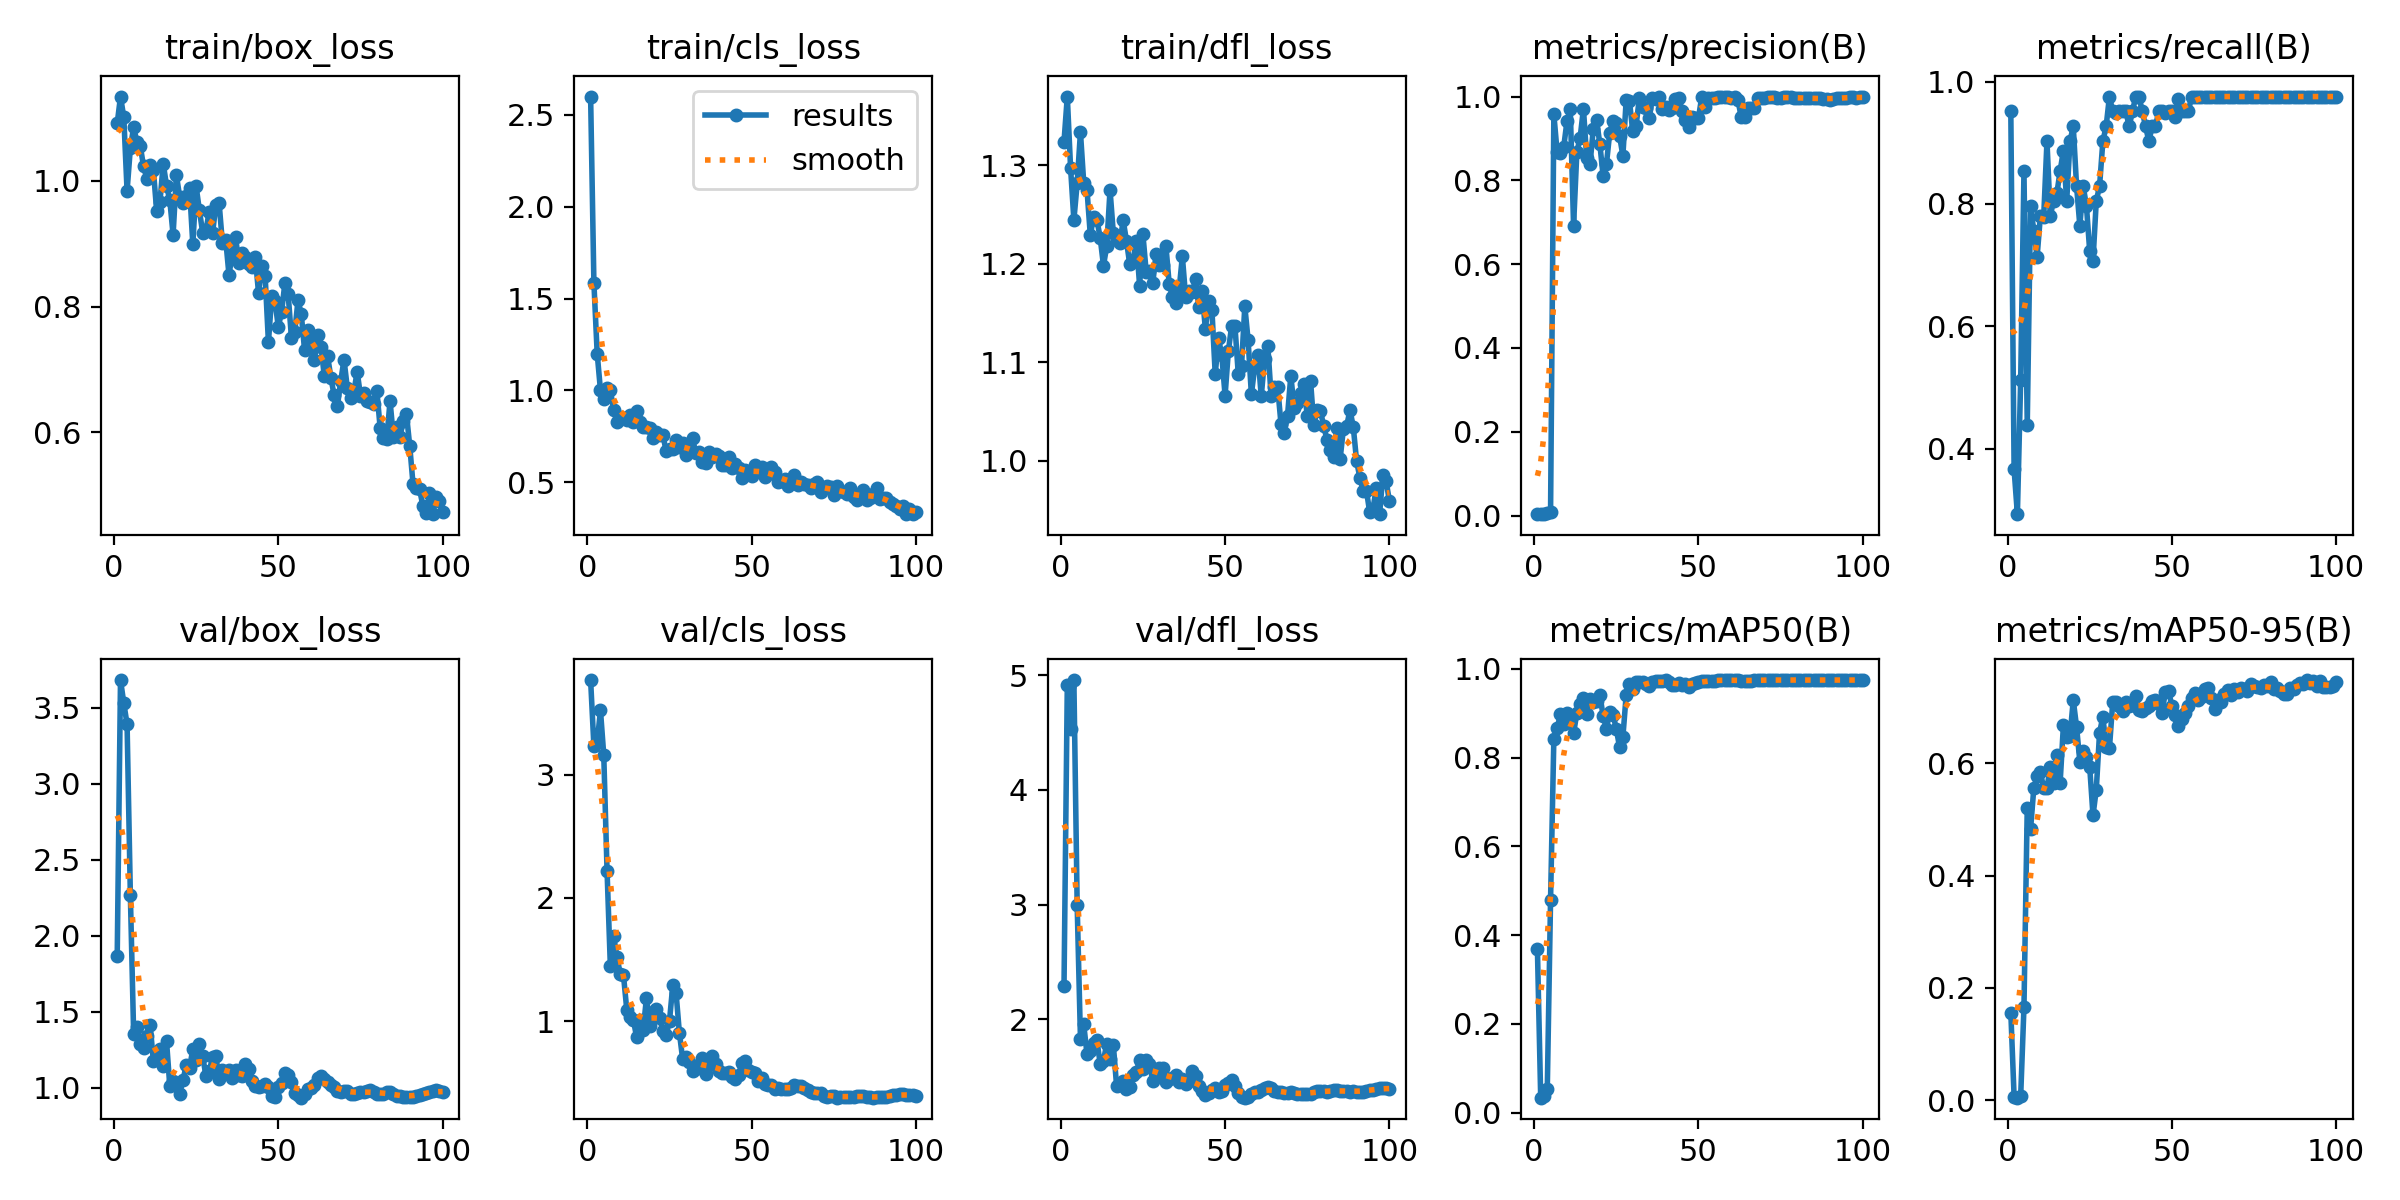
\includegraphics[width=0.92\columnwidth]{phone_results.png}
\captionof{figure}{Đường cong huấn luyện mô hình phát hiện điện thoại}
\label{fig:training_curves}
\end{minipage}

\vspace{6pt}
\noindent
\begin{minipage}{\columnwidth}
\centering
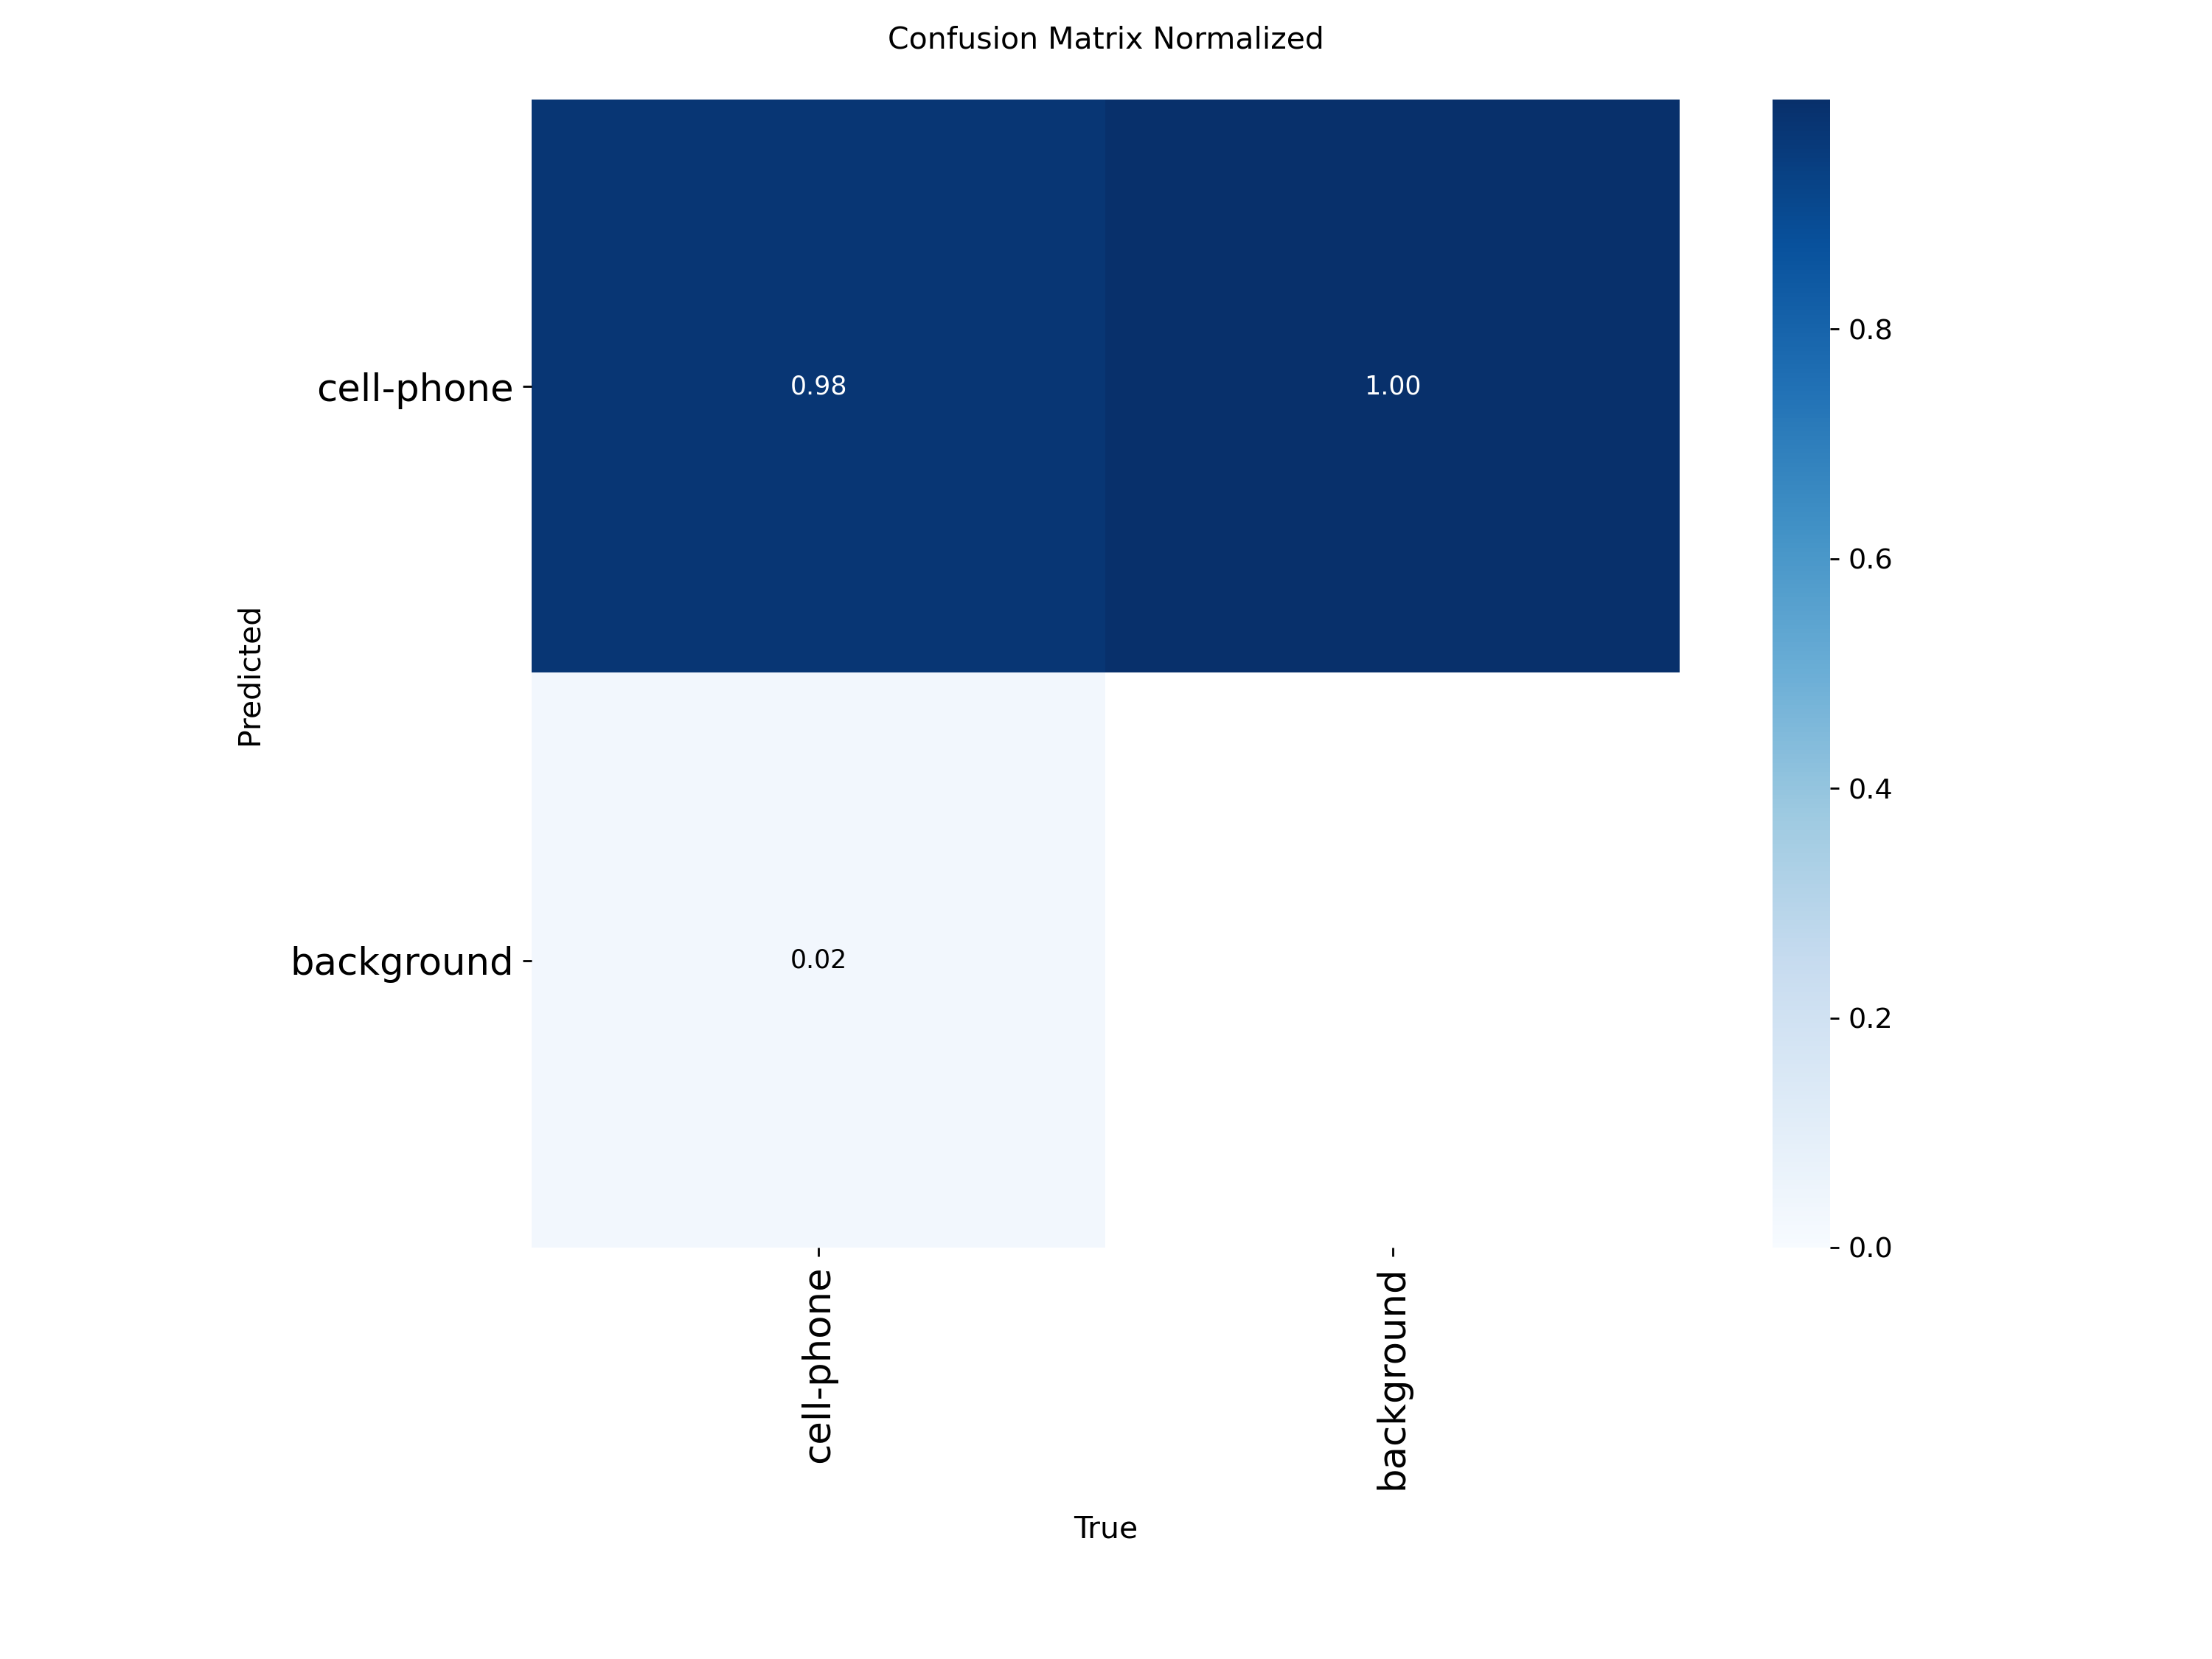
\includegraphics[width=0.82\columnwidth]{phone_confusion.png}
\captionof{figure}{Ma trận nhầm lẫn của mô hình phát hiện điện thoại}
\label{fig:confusion_matrix}
\end{minipage}
\vspace{6pt}

\subsection{Phát hiện dây an toàn}

Module sử dụng YOLOv8 được huấn luyện tùy chỉnh (trọng số {\tt day\_an\_toan.pt}) trên tập dữ liệu 1.200 ảnh thu thập từ nhiều góc nhìn trong cabin, áp dụng transfer learning với fine-tuning. Kết quả (Bảng~\ref{tab:yolo_training}) đạt mAP@50 = 0,753 và mAP@50--95 = 0,354 sau 50 epoch. Độ chính xác thấp hơn so với mô hình điện thoại do kích thước tập dữ liệu nhỏ hơn và sự đa dạng về tư thế, góc nhìn của dây an toàn.

\begin{figure}[H]
\centering

\includegraphics[width=\columnwidth]{images/dan.png}
\caption{Kết quả nhận diện tài xế trong thực nghiệm}
\label{fig:detection_examples}
\end{figure}

\begin{table}[H]
\centering
\caption{Kết quả huấn luyện các mô hình YOLO}
\fontsize{7}{8.5}\selectfont
\setlength{\tabcolsep}{2.5pt}
\resizebox{\columnwidth}{!}{%
\begin{tabular}{lcccc}
\toprule
Mô hình & Dữ liệu & Số ảnh & mAP@50 & mAP@50--95 \\
\midrule
CellPhone-YOLOv8n & COCO + In-Cabin Real & 8.500 & 0,975 & 0,748 \\
Seatbelt-YOLOv8 & Custom In-Cabin & 1.200 & 0,753 & 0,354 \\
\bottomrule
\end{tabular}
}
\label{tab:yolo_training}
\end{table}

\subsection{Hệ thống giao tiếp hai chiều AI--Web}

Luồng giao tiếp hai chiều (two-way communication) được tổ chức giữa ba tầng chuẩn: module AI suy luận (thuộc tầng ứng dụng) xử lý video với cơ chế tải mô hình lười biếng an toàn đa luồng; backend Flask ở tầng ứng dụng cung cấp REST API, WebSocket thời gian thực và MQTT cho kết nối IoT; dashboard web ở tầng giao diện thực hiện giám sát, hiển thị video stream, thống kê cảnh báo và lịch sử vi phạm. Cơ chế two-way communication cho phép hệ thống gửi cảnh báo, video stream đến web và web gửi lệnh bật/tắt module, điều chỉnh ngưỡng đến hệ thống.

Pipeline xử lý AI hoạt động tuần tự qua các module phát hiện. Mỗi module có thể bật/tắt độc lập. Cơ chế tổng hợp cảnh báo đa module theo mức ưu tiên với thời gian cooldown riêng. Cảnh báo được truyền qua ba kênh: âm thanh (pygame), hiển thị trên video stream, và thời gian thực qua WebSocket/MQTT.

\section{Thực nghiệm và kết quả}

\subsection{Thiết lập thực nghiệm}

Hệ thống được kiểm thử trên hai cấu hình: GPU (Intel Core i7-12700H, NVIDIA RTX 3050 Ti) và CPU (Intel Core i7-1165G7, Intel Iris Xe). Camera webcam độ phân giải 640$\times$480 ở 20 FPS, YOLOv8 chạy đầu vào 640$\times$640. Đánh giá gồm ba mức tách biệt: (1) chỉ số (i) mAP@50/mAP@50--95 trên tập huấn luyện Bảng~\ref{tab:yolo_training}: module điện thoại dùng 8.500 ảnh COCO kết hợp cabin, module dây an toàn dùng 1.200 ảnh cabin tùy chỉnh); (2) kiểm thử chức năng từng module trong phòng lab trên CPU với video cabin (độ chính xác phân loại, Bảng~\ref{tab:inference}); (3) kiểm thử toàn hệ thống end-to-end trên luồng webcam trực tiếp (độ chính xác cảnh báo và FPS/độ trễ, Bảng~\ref{tab:comparison}). Thời gian suy luận được đo bằng cơ chế timing instrumentation ghi log mỗi 100 frame.

\subsection{Kết quả và đánh giá}

Hệ thống có cơ chế đo thời gian suy luận (timing instrumentation) ghi log mỗi 100 frame. Bảng~\ref{tab:thresholds} liệt kê các tham số ngưỡng phát hiện của từng module.

Việc lựa chọn ngưỡng ảnh hưởng trực tiếp đến độ chính xác và tốc độ phát hiện. Ngưỡng EAR = 0,30 kết hợp với thời gian nhắm mắt tối thiểu 2 giây giúp phân biệt chớp mắt tự nhiên (100--400~ms) với buồn ngủ thực sự, giảm dương tính giả. Ngưỡng YAWN = 25~pixel và 15 khung hình liên tiếp (tương đương 0,75~giây ở 20~FPS) loại bỏ các chuyển động miệng ngắn (nói chuyện, cười). Ngưỡng tư thế đầu $|yaw| > 40^\circ$ và $pitch > 35^\circ$ theo biên độ nhìn tự nhiên khi lái xe \cite{lawson2020}; conf $>0,5$ cho YOLO để cân bằng precision--recall; FistScore $\geq 3$ (cơ chế đa số với 4/5 ngón) cân bằng giữa độ nhạy và độ đặc hiệu. Cơ chế cooldown (2--4~giây) ngăn cảnh báo trùng lặp, giảm nhiễu cho người lái.

\begin{table}[H]
\centering
\caption{Tham số ngưỡng phát hiện các module}
\fontsize{7}{8.5}\selectfont
\setlength{\tabcolsep}{2.5pt}
\begin{tabular}{llr}
\toprule
Module & Tham số & Giá trị \\
\midrule
Phát hiện nhắm mắt & EAR\_THRESHOLD & 0,30 \\
 & EAR\_MIN\_DURATION & 2 giây \\
Phát hiện ngáp & YAWN\_THRESHOLD & 25 pixel \\
 & YAWN\_CONSEC\_FRAMES & 15 khung hình \\
Tư thế đầu & Ngưỡng yaw & $>40^\circ$ \\
 & Ngưỡng pitch & $>35^\circ$ \\
Điện thoại & Confidence & $>0,5$ \\
Dây an toàn & Confidence & $>0,5$ \\
Tay lái & warning\_duration & 3 giây \\
 & FistScore & $\geq 3$ \\
\midrule
Cooldown & eye/yawn/head/phone & 2--3 giây \\
 & seatbelt/hand & 4 giây \\
\bottomrule
\end{tabular}
\label{tab:thresholds}
\end{table}

\begin{table}[H]
\centering
\caption{Mức ưu tiên và hành động xử lý cảnh báo}
\fontsize{7}{8.5}\selectfont
\setlength{\tabcolsep}{2.5pt}
\begin{tabular}{llcc}
\toprule
Module & Mức & Âm thanh & Kênh truyền \\
\midrule
Nhắm mắt & critical & nham\_mat.wav & WebSocket + MQTT \\
Điện thoại & critical & not\_phone.wav & WebSocket + MQTT \\
Dây an toàn & critical & seatbelt\_alert.wav & WebSocket + MQTT \\
Ngáp & warning & ngap\_ngu.wav & WebSocket \\
Mất tập trung & warning & dau\_quay.wav & WebSocket \\
Tay lái & warning & tay\_lai\_xe.wav & WebSocket \\
\bottomrule
\end{tabular}
\label{tab:priority}
\end{table}

Bảng~\ref{tab:inference} trình bày thời gian suy luận và độ chính xác phân loại của từng module trong kiểm thử lab trên CPU với độ phân giải 640$\times$480. Pipeline xử lý tuần tự trên CPU đạt 2,16 FPS (462,37 ms/frame), trong đó các mô hình YOLOv8 chiếm phần lớn thời gian xử lý.

\vspace{6pt}
\noindent
\begin{minipage}{\columnwidth}
\centering
\captionof{table}{Hiệu năng suy luận và độ chính xác phân loại của các mô-đun trong kiểm thử lab trên CPU.}
\label{tab:inference}
\fontsize{7}{8.5}\selectfont
\setlength{\tabcolsep}{2.5pt}
\resizebox{\columnwidth}{!}{%
\begin{tabular}{lrrr}
\toprule
Mô-đun & Thời gian (ms) & FPS & Độ chính xác phân loại lab (\%) \\
\midrule
Phát hiện khuôn mặt và điểm mốc (dlib) & 51,96 & 19,24 & 95,0 \\
Phát hiện điện thoại (YOLOv8n-custom) & 173,23 & 5,77 & 99,8 \\
Phát hiện dây an toàn (YOLOv8-custom) & 153,92 & 6,49 & 80,7 \\
Ước lượng tư thế (MediaPipe) & 83,26 & 12,01 & 90,5 \\
Toàn bộ hệ thống & 462,37 & 2,16 & 89,9 \\
\bottomrule
\end{tabular}
}
\end{minipage}
\vspace{6pt}

Độ chính xác của từng module chịu ảnh hưởng trực tiếp từ ngưỡng phát hiện. dlib đạt 95,0\% nhờ HOG+SVM phát hiện khuôn mặt chính diện ổn định, nhưng giảm khi góc nghiêng vượt $30^\circ$. YOLOv8n phát hiện điện thoại đạt precision 99,8\% ở ngưỡng conf $>0,5$ trên tập kiểm thử -- đây là độ chính xác phân loại, khác với tỷ lệ phát hiện thực tế ngoài cabin (khoảng 55\% do khác biệt góc camera và ánh sáng so với tập COCO). YOLOv8 phát hiện dây an toàn đạt 80,7\% với conf $>0,5$, thấp hơn do tập huấn luyện chỉ 1.200 ảnh. MediaPipe đạt 90,5\% nhờ mô hình TFLite nhẹ hoạt động ổn định trong cabin. Giá trị trung bình 89,9\% trong bảng này là kết quả lab trên CPU, phản ánh sự cân bằng giữa độ nhạy và độ đặc hiệu ở các ngưỡng đã chọn. Về thời gian, hai mô hình YOLOv8 chiếm $\sim$71\% tổng thời gian xử lý (327~ms), cho thấy đây là nút thắt cổ chai cần tối ưu.

Trên luồng webcam trực tiếp, hệ thống đạt tốc độ 20--30 FPS với độ trễ 100--200 ms và độ chính xác end-to-end khoảng 92\% trên GPU, trong khi trên CPU chỉ đạt 2--5 FPS với độ trễ 200--500 ms và khoảng 85\% chênh lệch do pipeline tuần tự trên CPU bỏ lỡ sự kiện khi tải YOLO cao, Bảng~\ref{tab:comparison}). GPU nhanh hơn 6--10 lần, khẳng định vai trò thiết yếu của tăng tốc phần cứng trong các hệ thống DMS đa module.

\begin{table}[H]
\centering
\caption{So sánh hiệu năng end-to-end trên luồng webcam trực tiếp (CPU vs GPU)}
\fontsize{7}{8.5}\selectfont
\setlength{\tabcolsep}{2.5pt}
\begin{tabular}{lrrr}
\toprule
Cấu hình & FPS & Độ trễ (ms) & Độ chính xác end-to-end \\
\midrule
CPU (i7-1165G7, Iris Xe) & 2--5 & 200--500 & $\sim$85\% \\
GPU (i7-12700H, RTX 3050 Ti) & 20--30 & 100--200 & $\sim$92\% \\
\bottomrule
\end{tabular}
\label{tab:comparison}
\end{table}

\section{Thảo luận}

Do trọng tâm của bài báo, chúng tôi tập trung thảo luận về camera như cảm biến chính để giám sát hành vi người lái. Giám sát người lái giải quyết việc phát hiện sớm các trường hợp mất tập trung hoặc có nguy cơ mất tập trung khỏi nhiệm vụ lái xe. Hai nguyên nhân chính là mệt mỏi (yếu tố không tự nguyện) và phân tâm (thường do cố ý). Cả hai đều yêu cầu khả năng thu thập và định vị đầu, khuôn mặt và mắt của người lái trong điều kiện khó khăn như chuyển động xe và ánh sáng thay đổi liên tục, dẫn đến bóng đổ hoặc phơi sáng quá mức \cite{voulodimos2018, lecun2015}.

Kết quả thực nghiệm cho thấy hệ thống đáp ứng tốt các mục tiêu về chức năng và hiệu năng. Hệ thống đạt tốc độ xử lý 20--30 FPS trên GPU, đáp ứng yêu cầu giám sát thời gian thực. Tuy nhiên, một số hạn chế cần được cải thiện:

\begin{itemize}[leftmargin=*,nosep]
  \item Hiệu năng trên CPU còn thấp (2--5 FPS) do pipeline tuần tự chưa tận dụng đa luồng.
  \item Độ chính xác phát hiện dây an toàn (80,7\%) cần cải thiện thông qua mở rộng tập dữ liệu.
  \item Chưa có đánh giá trên bộ dữ liệu chuẩn công khai như Drive\&Act.
  \item Giao diện web dùng polling thay vì WebSocket gây độ trễ hiển thị cảnh báo.
\end{itemize}

\section{Kết luận và hướng phát triển}

Bài báo đã trình bày một hệ thống giám sát tài xế thông minh ứng dụng AI với kiến trúc đa module tích hợp sáu thành phần phát hiện hành vi tài xế: buồn ngủ (dlib EAR), ngáp (facial landmarks), tư thế đầu (PnP), điện thoại (YOLOv8n), dây an toàn (YOLOv8 custom) và tay lái (MediaPipe). Hệ thống được tổ chức theo kiến trúc ba tầng truyền thống (giao diện--ứng dụng--dữ liệu), trong đó tầng ứng dụng tích hợp module AI suy luận chuyên biệt với cơ chế tải mô hình lười biếng an toàn đa luồng, hàng đợi cảnh báo và cảnh báo đa kênh (âm thanh, WebSocket, MQTT).

Kết quả thực nghiệm trên GPU (RTX 3050 Ti) cho thấy hệ thống đáp ứng yêu cầu giám sát thời gian thực với tốc độ xử lý 20--30 FPS, độ trễ đầu cuối 100--200 ms.

Hướng phát triển trong tương lai:
\begin{itemize}[leftmargin=*,nosep]
  \item Triển khai Edge AI: Chuyển pipeline lên NVIDIA Jetson Nano với TensorRT để tối ưu inference, giảm chi phí phần cứng.
  \item Mô hình tiên tiến: Nâng cấp lên YOLOv10/v11, áp dụng Transformer cho phân tích chuỗi hành vi phức tạp \cite{nimma2025}.
  \item Mở rộng dữ liệu: Thu thập thêm dữ liệu đa dạng về điều kiện ánh sáng, góc nhìn và đối tượng người lái.
  \item Tối ưu pipeline: Chuyển sang xử lý đa luồng và pipeline bất đồng bộ.
\end{itemize}

\subsection*{Lời cảm ơn}
Nghiên cứu này được tài trợ bởi Trường Đại học Công nghệ Giao thông vận tải (UTT), mã số đề tài: ĐTSV2526-280. Nhóm tác giả chân thành cảm ơn các cộng tác viên đã hỗ trợ thu thập dữ liệu và đánh giá thử nghiệm hệ thống.

\begin{thebibliography}{99}
\fontsize{9}{11}\selectfont
\raggedright
\color{jsttcite}

\bibitem{hien2026} Hiến, Đ. (2026). \textit{Báo cáo ATGT Quốc gia giai đoạn 2024--2025}. Ủy ban An toàn giao thông Quốc gia.

\bibitem{aaa2018} AAA Foundation for Traffic Safety. (2018). Acute sleep deprivation and risk of motor vehicle crash involvement. \textit{AAA NewsRoom}.

\bibitem{soukupova2016} Soukupova, T., \& Cech, J. (2016). Eye blink detection using facial landmark tracking. In \textit{Proceedings of the International Conference on Computer Vision Theory and Applications (VISAPP)} (Vol.~2, pp.~328--335).

\bibitem{king2009} King, D. E. (2009). Dlib-ml: A machine learning toolkit. \textit{Journal of Machine Learning Research}, 10, 1755--1758.

\bibitem{lawson2020} Lawson, A., Kim, J., \& Lee, T. (2020). Head pose estimation for driver distraction detection. \textit{IEEE Transactions on Intelligent Transportation Systems}, 21(7), 2964--2973.

\bibitem{redmon2016} Redmon, J., Divvala, S., Girshick, R., \& Farhadi, A. (2016). You only look once: Unified, real-time object detection. In \textit{Proceedings of the IEEE Conference on Computer Vision and Pattern Recognition (CVPR)} (pp.~779--788).

\bibitem{jocher2023} Jocher, G., Chaurasia, A., \& Qiu, J. (2023). \textit{YOLOv8 by Ultralytics} [Computer software]. GitHub.

\bibitem{lugaresi2019} Lugaresi, C., et al. (2019). MediaPipe: A framework for building perception pipelines. \textit{arXiv preprint arXiv:1906.08172}.

\bibitem{ji2002} Ji, Q., \& Yang, X. (2002). Real-time eye, gaze, and face pose tracking for monitoring driver vigilance. \textit{Real-Time Imaging}, 8(5), 357--377.

\bibitem{voulodimos2018} Voulodimos, A., et al. (2018). Deep learning for computer vision: A brief review. \textit{Computational Intelligence and Neuroscience}, 2018.

\bibitem{lecun2015} LeCun, Y., Bengio, Y., \& Hinton, G. (2015). Deep learning. \textit{Nature}, 521(7553), 436--444.

\bibitem{ngxande2017} Ngxande, M., Tapamo, J., \& Burke, M. (2017). Driver drowsiness detection: A review. In \textit{Proceedings of the IEEE AFRICON Conference} (pp.~991--996).

\bibitem{malek2021} Malek, S., et al. (2021). Head pose estimation using facial-landmarks classification for rehabilitation games. \textit{Pattern Recognition Letters}.

\bibitem{nimma2025} Nimma, D., et al. (2025). Object detection in real-time video surveillance using attention based Transformer-YOLOv8 model.

\bibitem{shorten2019} Shorten, C., \& Khoshgoftaar, T. (2019). A survey on image data augmentation for deep learning. \textit{Journal of Big Data}, 6(1), 1--48.

\bibitem{seeingmachines2022} Seeing Machines. (2022). \textit{Guardian DMS: Driver Monitoring System OEM} [Technical documentation].

\bibitem{veres2019} Veres, M., \& Moussa, M. (2019). Deep learning for intelligent transportation systems: A survey. \textit{IEEE Transactions on Intelligent Transportation Systems}, 21(11), 4602--4620.

\bibitem{zhou2025} Zhou, K. C., et al. (2025). Human pose prediction based on LSTM và MediaPipe. \textit{Tạp chí Khoa học và Công nghệ Kỹ thuật}.

\bibitem{baogiaothong2025} Báo Giao thông. (2025). Thống kê tai nạn giao thông tại Việt Nam. \textit{Báo Giao thông}.

\bibitem{minhvt2020} Minh, V. T. (2020). Chatbot tư vấn luật giao thông sử dụng RAG và Groq API. \textit{Tạp chí Khoa học và Công nghệ Giao thông}.

\end{thebibliography}

\end{multicols}
\end{document}